\documentclass[12pt,addpoints]{evalua}
\grado{1$^\circ$ de Secundaria}
\cicloescolar{2023-2024}
\materia{Matemáticas 1}
\unidad{1}
\title{Examen Extraordinario}
\aprendizajes{
        \item Convierte fracciones decimales a notación decimal y viceversa. Aproxima algunas fracciones no decimales usando la notación decimal. 
        \item Ordena fracciones y números decimales.
        \item Resuelve problemas de suma y resta con números enteros, fracciones y decimales positivos y negativos.
        \item Resuelve problemas de multiplicación con fracciones y decimales y de división con decimales.
}
     \author{Prof.: Julio César Melchor Pinto}
\begin{document}
\begin{questions}
    \section*{\ifprintanswers{Cálculos numéricos}\else{}\fi}

    \question[10] Realiza las siguientes operaciones de \textit{cálculo numérico}:
    \begin{parts}
        \begin{multicols}{2}
            \subsection*{\ifprintanswers{Suma de números}\else{}\fi}
            \part $\dfrac{5}{6}+\dfrac{3}{8}=$ \fillin[$1\dfrac{5}{24}$][0in]
            \subsection*{\ifprintanswers{Multiplicación de números}\else{}\fi}
            \part $9.27\times 5.4=$ \fillin[$50.058$][0in]
            \subsection*{\ifprintanswers{Resta de números}\else{}\fi}
            \part $\dfrac{1}{2}-\dfrac{2}{5}=$ \fillin[$\dfrac{1}{10}$][0in]
            \subsection*{\ifprintanswers{División de números}\else{}\fi}
            \part $622.21\divisionsymbol 115=$ \fillin[$5.41$][0in]
        \end{multicols}
        \subsection*{\ifprintanswers{Resolución de problemas}\else{}\fi}
        \part Si un dólar equivale a 19 pesos. ¿Cuántos dólares serán 1634 pesos? \fillin[$1634\divisionsymbol 19 =$ 86 dólares][0in]
    \end{parts}

    \newpage
    \section*{\ifprintanswers{Fracciones}\else{}\fi}

    \subsection*{\ifprintanswers{Clasificación de fracciones}\else{}\fi}

    \question[8] Clasifica las siguientes fracciones en propias, impropias o mixtas:
    \begin{multicols}{2}
        \begin{parts}
            \part $\dfrac{5}{6}=$ \fillin[Propia][1in]   \\
            \part $5\dfrac{5}{11}=$ \fillin[Mixta][1in]  \\
            \part $\dfrac{7}{3}=$ \fillin[Impropia][1in] \\
            % \part $\dfrac{3}{4}=$ \fillin[Propia][1in]   \\
            % \part $1\dfrac{2}{3}=$ \fillin[Mixta][1in]   \\
            % \part $\dfrac{7}{5}=$ \fillin[Impropia][1in] \\
            % \part $\dfrac{7}{8}=$ \fillin[Propia][1in] \\
            % \part $3\dfrac{2}{9}=$ \fillin[Mixta][1in]   \\
            \part $\dfrac{3}{2}=$ \fillin[Impropia][1in]   \\
            % \part $4\dfrac{1}{4}=$ \fillin[Mixta][1in] \\
        \end{parts}
    \end{multicols}
    \subsection*{\ifprintanswers{Representación de fracciones}\else{}\fi}
    \question[4] Escribe sobre la línea la fracción que representa cada imagen:
    \begin{multicols}{2}
        \begin{parts}
            \part 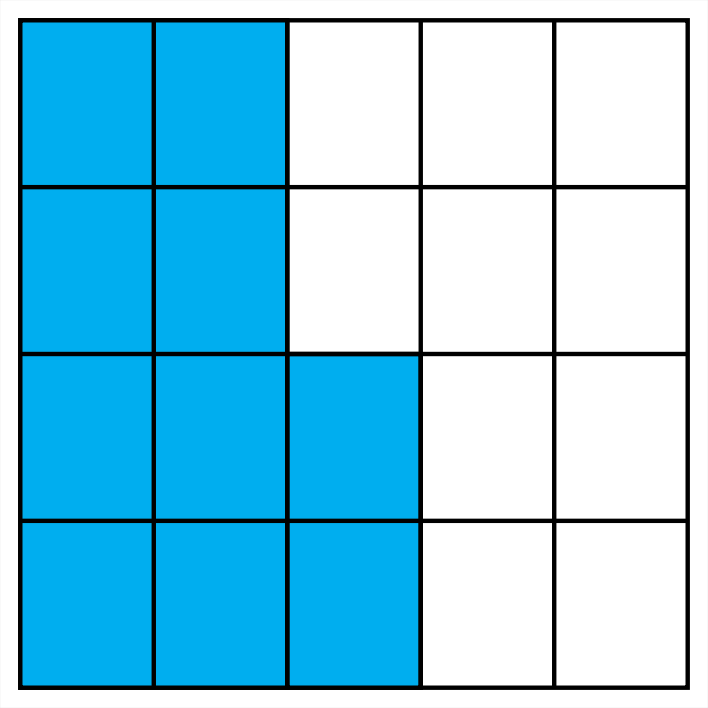
\includegraphics[width=80px]{../images/imagen_frac01.png} \fillin[$\dfrac{10}{20}$][1in]
            \part 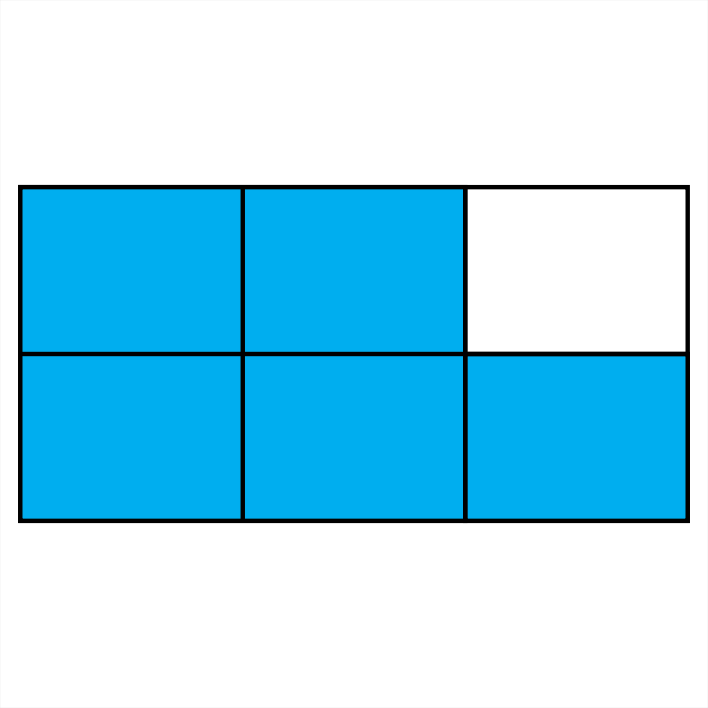
\includegraphics[width=80px]{../images/imagen_frac02.png} \fillin[$\dfrac{5}{6}$][1in]
            % \part 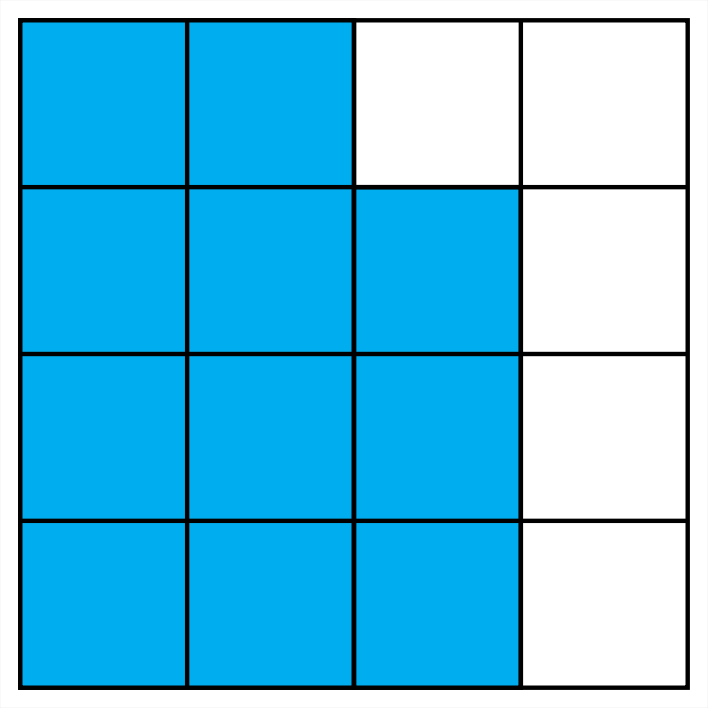
\includegraphics[width=100px]{../images/imagen_frac03.png} \fillin[$\dfrac{10}{20}$][1in]
            % \part 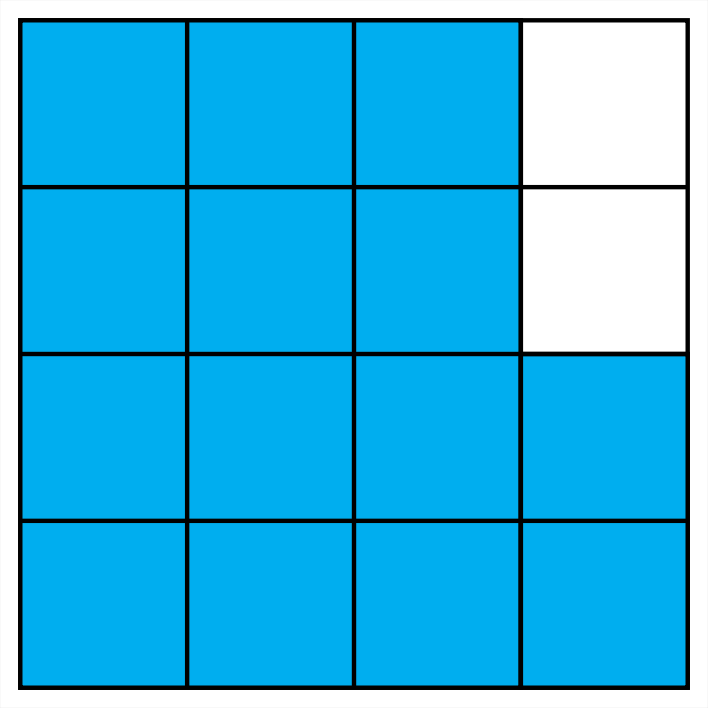
\includegraphics[width=100px]{../images/imagen_frac04.png} \fillin[$\dfrac{10}{20}$][1in]
            % \part 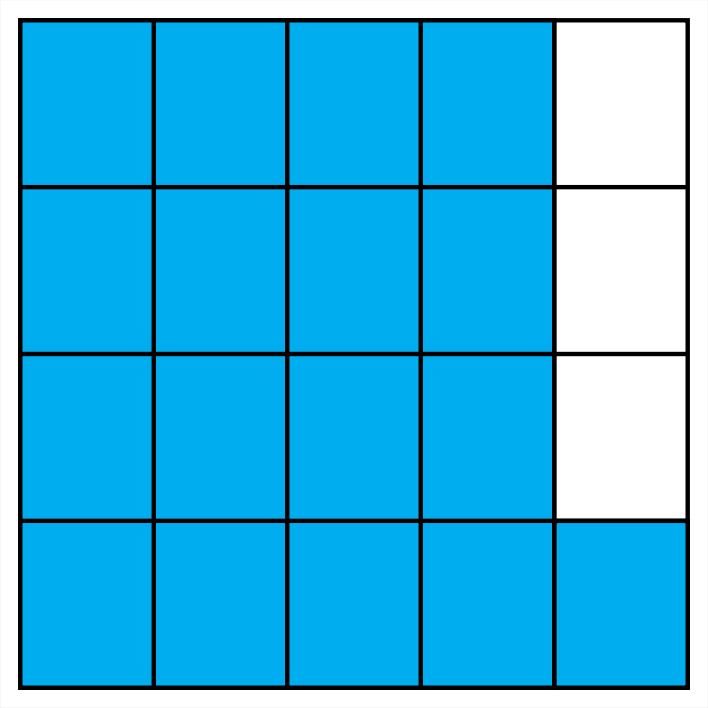
\includegraphics[width=100px]{../images/imagen_frac05.png} \fillin[$\dfrac{10}{20}$][1in]
            % \part 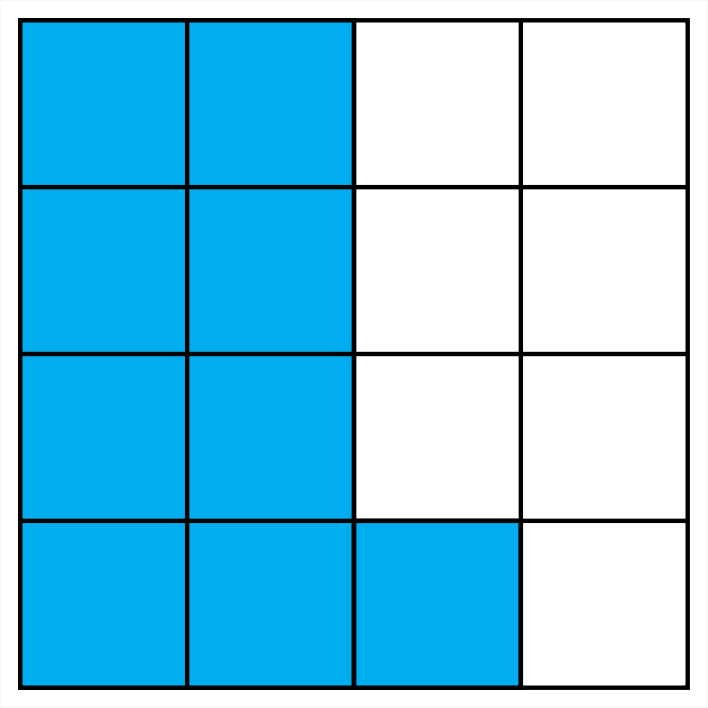
\includegraphics[width=100px]{../images/imagen_frac06.png} \fillin[$\dfrac{10}{20}$][1in]
            % \part 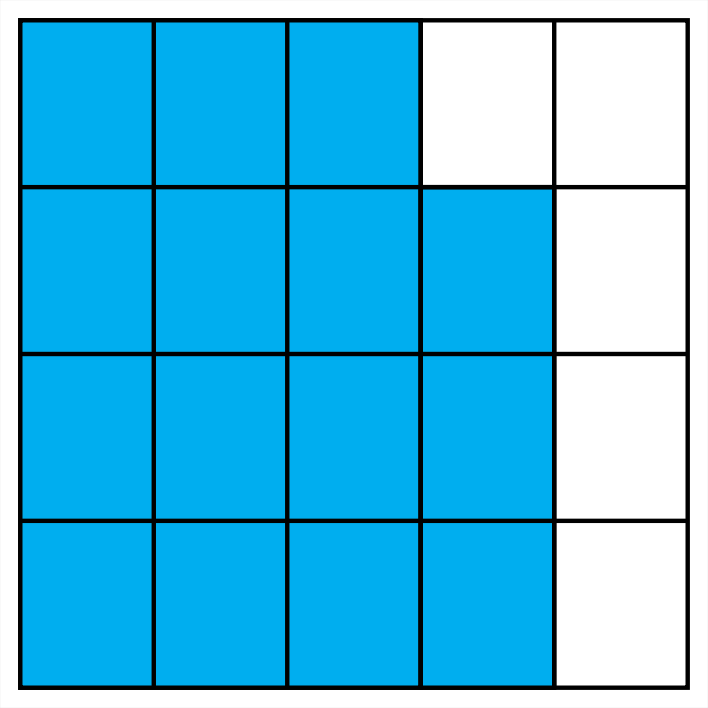
\includegraphics[width=100px]{../images/imagen_frac07.png} \fillin[$\dfrac{10}{20}$][1in]
            % \part 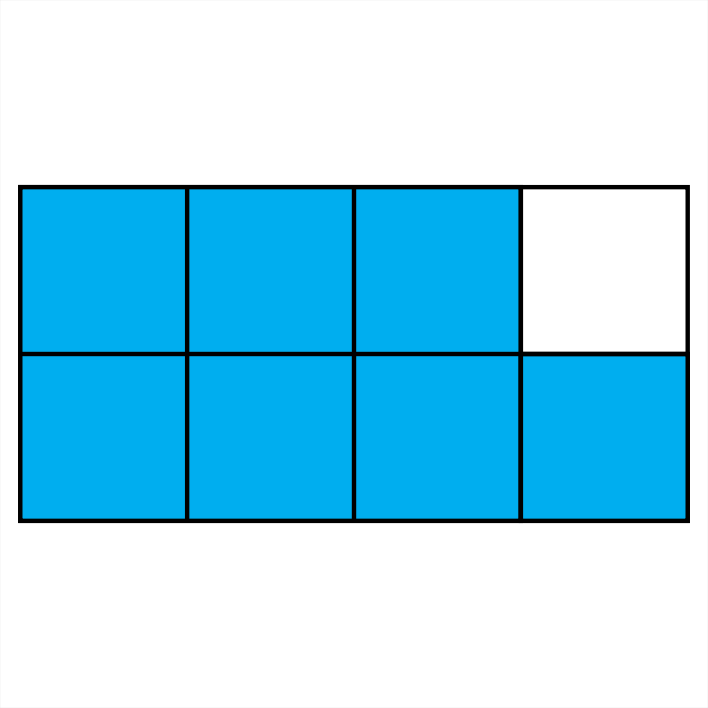
\includegraphics[width=100px]{../images/imagen_frac08.png} \fillin[$\dfrac{10}{20}$][1in]
            % \part 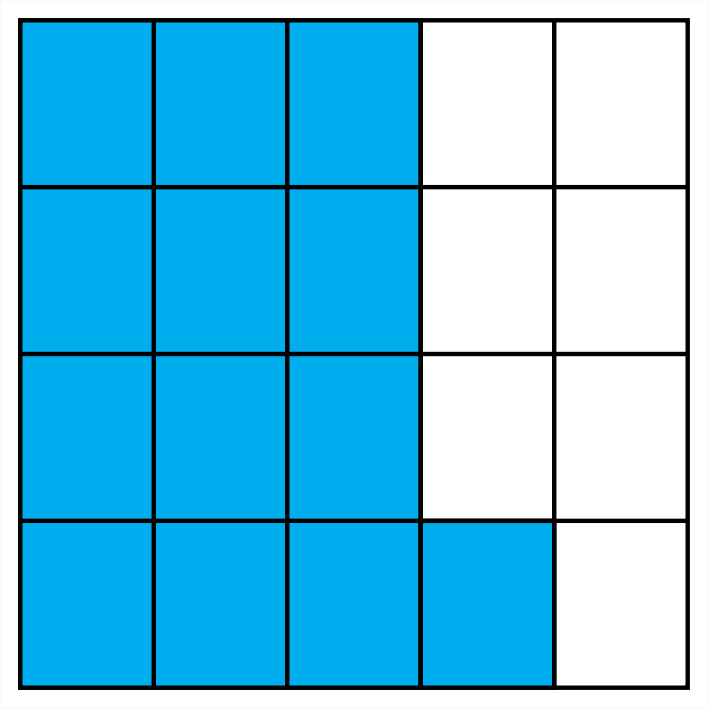
\includegraphics[width=100px]{../images/imagen_frac09.png} \fillin[$\dfrac{10}{20}$][1in]
            % \part 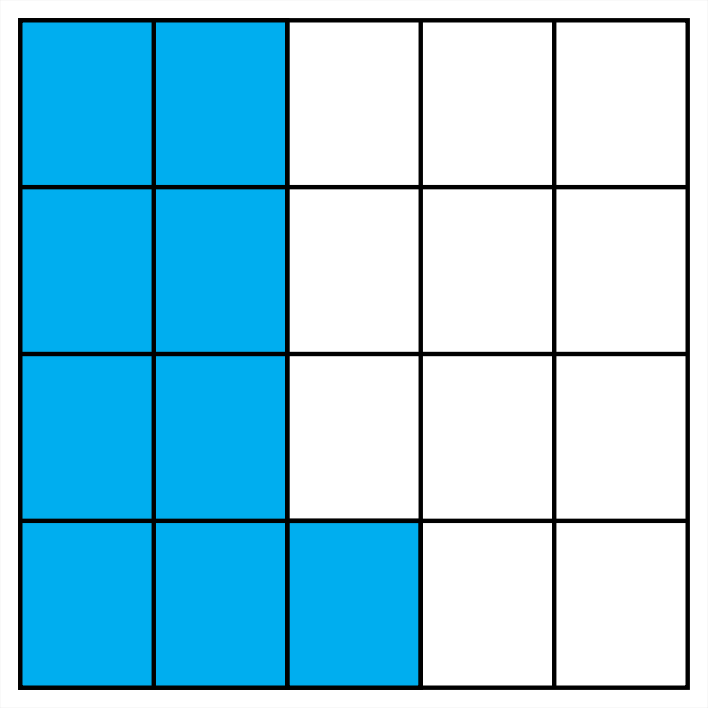
\includegraphics[width=100px]{../images/imagen_frac10.png} \fillin[$\dfrac{10}{20}$][1in]
        \end{parts}
    \end{multicols}

    \subsection*{\ifprintanswers{Nombre de fracciones}\else{}\fi}

    \question[4] Escribe la fracción que corresponda en cada inciso:
    \begin{parts}
        % \part ¿Cómo se escribe numéricamente la fracción \textbf{ocho quintos}?    \fillin[$\dfrac{8}{5}$][0in]  \\
        \part ¿Cómo se escribe numéricamente la fracción \textbf{seis onceavos}?   \fillin[$\dfrac{6}{11}$][0in] \\
        % \part ¿Cómo se escribe numéricamente la fracción \textbf{dos séptimos}?    \fillin[$\dfrac{2}{7}$][0in]  \\
        \part ¿Cómo se escribe numéricamente la fracción \textbf{once medios}?     \fillin[$\dfrac{11}{2}$][0in] \\
        % \part ¿Cómo se escribe numéricamente la fracción \textbf{diez décimos}?    \fillin[$\dfrac{10}{10}$][0in]\\
    \end{parts}

    \subsection*{\ifprintanswers{Fracciones en la recta numérica}\else{}\fi}

    \question[4] Escribe la fracción que representa el punto en la recta numérica
    \begin{multicols}{2}
        \begin{parts}
            \part 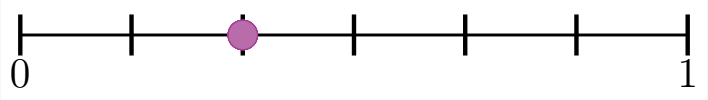
\includegraphics[width=150px]{../images/recta_num_frac01.png} \\[-0.5em] \fillin[$\dfrac{2}{6}$][2in]
            \part 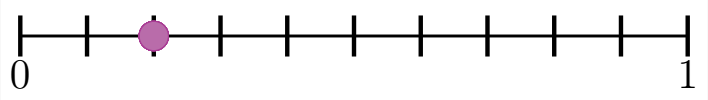
\includegraphics[width=150px]{../images/recta_num_frac02.png} \\[-0.5em] \fillin[$\dfrac{2}{10}$][2in]
            % \part 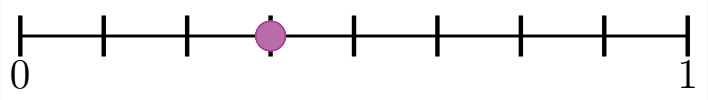
\includegraphics[width=150px]{../images/recta_num_frac03.png} \\[-0.5em] \fillin[$\dfrac{2}{6}$][1.5in]
            % \part 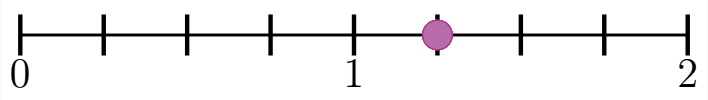
\includegraphics[width=150px]{../images/recta_num_frac04.png} \\[-0.5em] \fillin[$\dfrac{2}{6}$][1.5in]
            % \part 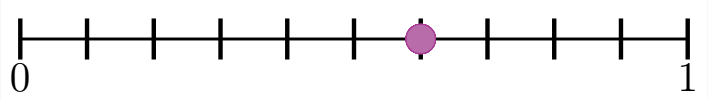
\includegraphics[width=150px]{../images/recta_num_frac05.png} \\[-0.5em] \fillin[$\dfrac{2}{6}$][1.5in]
            % \part 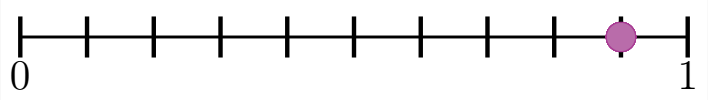
\includegraphics[width=150px]{../images/recta_num_frac06.png} \\[-0.5em] \fillin[$\dfrac{2}{6}$][1.5in]
            % \part 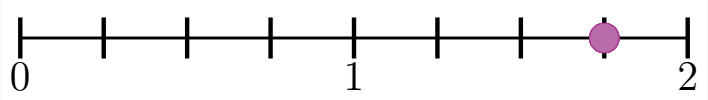
\includegraphics[width=150px]{../images/recta_num_frac07.png} \\[-0.5em] \fillin[$\dfrac{2}{6}$][1.5in]
            % \part 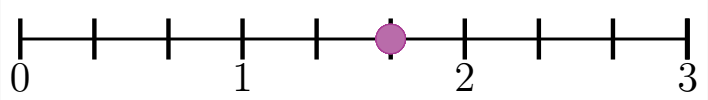
\includegraphics[width=150px]{../images/recta_num_frac08.png} \\[-0.5em] \fillin[$\dfrac{2}{6}$][1.5in]
            % \part 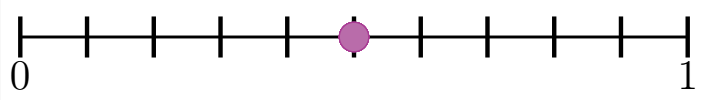
\includegraphics[width=150px]{../images/recta_num_frac09.png} \\[-0.5em] \fillin[$\dfrac{2}{6}$][1.5in]
            % \part 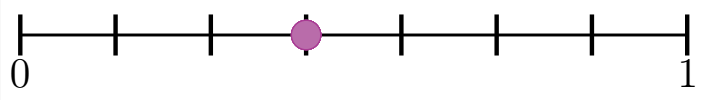
\includegraphics[width=150px]{../images/recta_num_frac10.png} \\[-0.5em] \fillin[$\dfrac{2}{6}$][1.5in]
        \end{parts}
    \end{multicols}

    \subsection*{\ifprintanswers{Conversión de fracciones}\else{}\fi}

    \question[4] Convierte la siguientes fracciones impropias a mixtas:
    \begin{multicols}{3}
        \begin{parts}
            \part $\dfrac{13}{3}= $ \fillin[$4\dfrac{1}{3}$][0in]
            % \part $\dfrac{63}{10}= $ \fillin[$6\dfrac{3}{10}$][0in]
            \part $\dfrac{51}{5}= $ \fillin[$10\dfrac{1}{5}$][0in]
        \end{parts}
    \end{multicols}

    \newpage
    \section*{\ifprintanswers{Fracciones, M.C.M. y M.C.D.}\else{}\fi}

    \subsection*{\ifprintanswers{Comparación de fracciones}\else{}\fi}

    \question[8] Compara las siguientes fracciones usando los signos mayor que (>), menor que (<) o igual (=):
    \begin{multicols}{3}
        \begin{parts}
            \part $\dfrac{4}{3}$ \fillin[$>$][0.5in] $\dfrac{5}{4}$\\[0.75em]
            \part $\dfrac{1}{3}$ \fillin[$=$][0.5in] $\dfrac{3}{9}$\\[0.75em]
            % \part $\dfrac{2}{3}$ \fillin[$<$][0.5in] $\dfrac{3}{2}$\\[0.75em]
            % \part $\dfrac{3}{4}$ \fillin[$>$][0.5in] $\dfrac{2}{3}$\\[0.75em]
            \part $\dfrac{5}{6}$ \fillin[$>$][0.5in] $\dfrac{4}{5}$\\[0.75em]
            \part $\dfrac{1}{3}$ \fillin[$<$][0.5in] $\dfrac{2}{5}$\\[0.75em]
        \end{parts}
    \end{multicols}

    \subsection*{\ifprintanswers{Fracciones equivalentes}\else{}\fi}
    \question[8] Indica si las siguientes fracciones son equivalentes o no:
    \begin{multicols}{2}
        \begin{parts}
            \part $\dfrac{4}{5}=\dfrac{8}{10}$\qquad
            \begin{oneparcheckboxes}
                \CorrectChoice Sí
                \choice No
            \end{oneparcheckboxes}

            \part $\dfrac{1}{8}=\dfrac{4}{16}$\qquad
            \begin{oneparcheckboxes}
                \choice Sí
                \CorrectChoice No
            \end{oneparcheckboxes}

            \part $\dfrac{1}{5}=\dfrac{5}{10}$\qquad
            \begin{oneparcheckboxes}
                \choice Sí
                \CorrectChoice No
            \end{oneparcheckboxes}

            \part $\dfrac{1}{10}=\dfrac{3}{30}$\qquad
            \begin{oneparcheckboxes}
                \CorrectChoice Sí
                \choice No
            \end{oneparcheckboxes}
        \end{parts}
    \end{multicols}

    \subsection*{\ifprintanswers{M.C.D y M.C.M}\else{}\fi}
    \question[4] Calcula lo que se te pide en cada inciso:
    \begin{parts}
        \part Encuentra el máximo común divisor de 33 y 121. \fillin[$\text{mcd}(33,121)=11$][0in]
        \part Encuentra el mínimo común múltiplo de 2, 3 y 4. \fillin[$\text{mcm}(2,3,4)=12$][0in]
    \end{parts}

    \subsection*{\ifprintanswers{Simplificación de fracciones}\else{}\fi}
    \question[4] Simplifica a su mínima expresión la siguiente fracción usando el máximo común divisor
    \begin{multicols}{2}
        \begin{parts}
            \part $\dfrac{8}{64}=$ \fillin[$\dfrac{1}{8}$][0in]
            \part $\dfrac{6}{42}=$ \fillin[$\dfrac{1}{7}$][0in]
        \end{parts}
    \end{multicols}

    \subsection*{\ifprintanswers{Resolución de problemas}\else{}\fi}

    \question[6] María y Jorge tienen 45 bolas blancas, 15 bolas azules y 90 bolas rojas y quieren hacer el mayor número de collares iguales sin que sobre ninguna bola. ¿Cuántos collares iguales pueden hacer?
    \begin{solutionbox}{4cm}
        Se calcula el M.C.D.$(45,15,90) = 15$.\\
        Por lo tanto, se pueden hacer 15 collares.
    \end{solutionbox}
    \newpage
    \section*{\ifprintanswers{Números decimales}\else{}\fi}

    \subsection*{\ifprintanswers{Ubicación en la recta numérica}\else{}\fi}

    \question[4] Escribe el número que representa el punto indicado en la recta numérica de cada uno de los siguientes incisos.

    \begin{multicols}{2}
        \begin{parts}
            \part 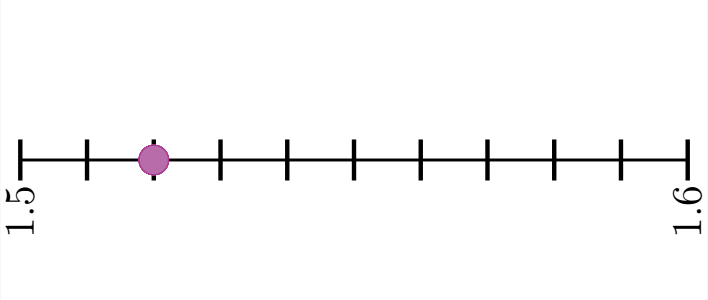
\includegraphics[width=150px]{../images/recta_num_1.52.png} \\[-0.5em] \fillin[$1.52$][1.5in]
            \part 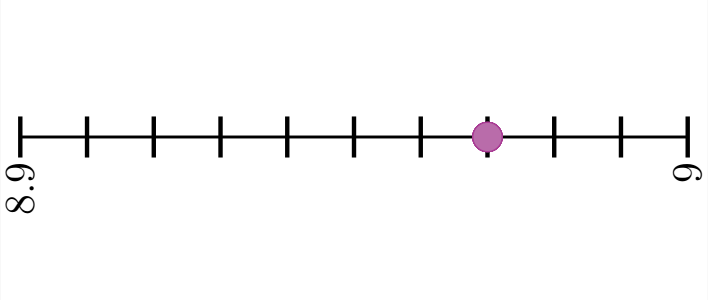
\includegraphics[width=150px]{../images/recta_num_8.97.png} \\[-0.5em]  \fillin[$8.97$][1.5in]  \\[-1.4em]
        \end{parts}
    \end{multicols}

    \subsection*{\ifprintanswers{Porcentajes a decimal}\else{}\fi}

    \question[4] Escribe el número decimal que representa cada porcentaje:

    \begin{multicols}{2}
        \begin{parts}
            \part Convierte 22.9\% a un número decimal. \fillin[$0.229$][0in]
            \part Convierte 6.2\% a un número decimal. \fillin[$0.062$][0in]
        \end{parts}
    \end{multicols}

    \subsection*{\ifprintanswers{Operaciones con múltiplos de 10}\else{}\fi}

    \question[4] Realiza las siguientes operaciones con múltiplos de 10:

    \begin{multicols}{2}
        \begin{parts}
            \part $56.9 \times 100=$ \fillin[$5690$][0in]
            \part $0.712 \times 1000=$ \fillin[$712$][0in]
        \end{parts}
    \end{multicols}


    \subsection*{\ifprintanswers{Conversión de fracciones a decimales}\else{}\fi}
    \question[4] Convierte las siguientes fracciones a decimales:
    \begin{multicols}{2}
        \begin{parts}
            \part $\dfrac{7}{20}=$ \fillin[$0.35$][0in]
            \part $\dfrac{1927}{1000}=$ \fillin[$1.927$][0in]
        \end{parts}
    \end{multicols}

    \subsection*{\ifprintanswers{Conversión de decimales a fracciones}\else{}\fi}
    \question[4] Convierte los siguientes números decimales a una fracción simplificada a su mínima expresión:
    \begin{multicols}{2}
        \begin{parts}
            \part $0.04=$ \fillin[$\dfrac{1}{25}$][0in]
            \part $0.19=$ \fillin[$\dfrac{19}{100}$][0in]
        \end{parts}
    \end{multicols}

    \newpage

    \section*{\ifprintanswers{Números negativos}\else{}\fi}
    \subsection*{\ifprintanswers{Ubicación en la recta numérica}\else{}\fi}
    \question[4] Escribe el número que representa el punto indicado en la recta numérica de cada uno de los siguientes incisos.

    \begin{multicols}{2}
        \begin{parts}
            \part 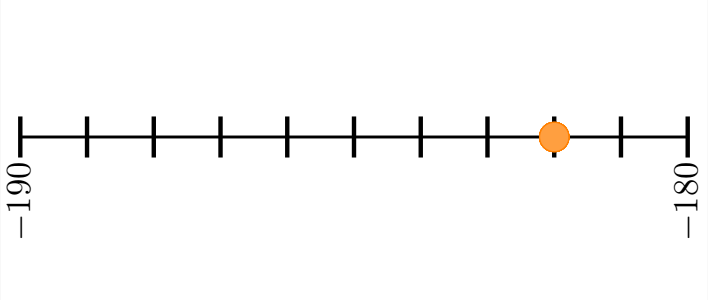
\includegraphics[width=150px]{../images/recta_num_-182.png} \\[-0.5em]   \fillin[$-182$][1.5in]
            \part 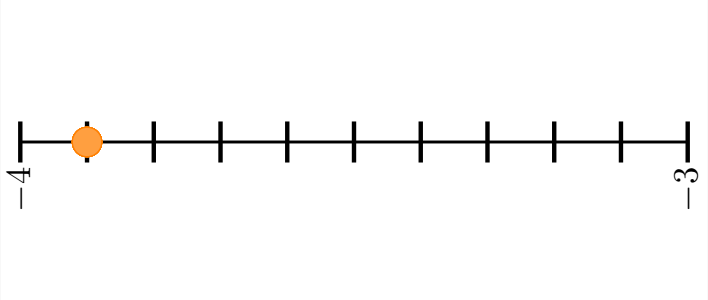
\includegraphics[width=150px]{../images/recta_num_-3.9.png} \\[-0.5em]  \fillin[$-3.9$][1.5in]
        \end{parts}
    \end{multicols}

    \subsection*{\ifprintanswers{Comparación de negativos}\else{}\fi}
    \question[4] Escribe sobre la línea el símbolo de mayor que ($>$), menor que ($<$), o igual ($=$) según corresponda.
    \begin{multicols}{2}
        \begin{parts}
            \part $-182$ \fillin[$>$][0.5in] $-189$\\[0.75em]
            \part $-97$ \fillin[$<$][0.5in] $-96.2$\\[0.75em]
        \end{parts}
    \end{multicols}

    \subsection*{\ifprintanswers{Determina el signo}\else{}\fi}
    \question[4] Determina el signo \textit{positivo} o \textit{negativo} que resulta de las siguientes operaciones:
    \begin{multicols}{2}
        \begin{parts}
            \part $-28-19$ \fillin[Negativo][1in]
            \part $-43+55$ \fillin[Positivo][1in]
        \end{parts}
    \end{multicols}

    \subsection*{\ifprintanswers{Suma y resta con negativos }\else{}\fi}
    \question[4] Realiza las siguientes operaciones con números negativos:
    \begin{multicols}{2}
        \begin{parts}
            \part $-223+67=$ \fillin[$-156$][0in]
            \part $(16)-(-14)$ \fillin[$30$][0in]
        \end{parts}
    \end{multicols}
\end{questions}
\end{document}